% Template for a Thesis
%
% 6-development.tex
%
% Development

\chapter{Development}\label{ch:development}

This chapter explains the development of the thesis in a deeper way, adding more detailed explanations, the code and algorithms previously explained in the Methodology section.~\ref{ch:methodology} This chapter includes coding practices, how global variables are stored and treated, the tree directory of the project, and the various tasks that have been undertaken during this thesis, which include the following:

\begin{enumerate}
  \item Replication of the BPE algorithm and results
  \item Replication of the BPE dropout algorithm and results
  \item Improvement of the learn BPE algorithm
  \item Study and implementation of BPE without word boundaries
\end{enumerate}

\section{Coding practices}

To ensure consistency, the parameters for the pipeline, called global variables, such as num\_symbols, dropout, file paths, etc. have been written in \emph{settings.py}. The word separator is a special Unicode character. The languages used as source and target languages are English and German respectively. The number of symbols to be learnt in the learn BPE phase is set as 20000. When applying these merges to the corpus, in order to have different variants and explore the differences between merging few symbols or more, a number of key numbers are selected for these experiments, as seen in the variable \emph{all\_symbols}.

\begin{python}
# settings.py
import os
import glob
from os.path import join

word_sep = u'\u2581'
source, target = 'eng', 'deu'
learn_symbols = 20000
all_symbols = [100, 200, 500, 1000, 2000, 4000, 6000, 8000]

rootdir = os.getcwd()
if rootdir.split(os.sep)[-1] == 'src':
    rootdir = os.sep.join(rootdir.split(os.sep)[:-1])
datadir = join(rootdir, 'data')
inputdir = join(datadir, 'input')
bpedir = join(datadir, 'normal_bpe')
baselinedir = join(rootdir, 'reports', 'scores_normal_bpe')
scoredir = join(rootdir, 'reports', 'scores_normal_bpe')
goldpath = join(inputdir, 'eng_deu.gold')
inputpath = {}
for filename in glob.glob(join(inputdir, "*.txt")):
  inputpath[filename.split(os.sep)[-1].split('_')[0]] = filename
\end{python}

Regarding directories and paths, the tree view of the project is displayed in the following figure. The input data is saved into \emph{data/input}, the rest of the intermediate data files such as \emph{.bpe}, \emph{.wgdfa} and others are saved into their respective folder depending on the dropout parameter. The models are saved in the general \emph{data} folder with the \emph{.model} extension. The LaTeX files for writing this thesis are saved in the \emph{doc} folder, the score figures and csv files in \emph{reports}, all Python scripts in \emph{src}, the \emph{Fastalign} and \emph{Eflomal} installation files in \emph{tools}, and README, requirements, gitignore and the global variable file \emph{settings.py} are saved in the root folder.

\begin{figure}[!ht]
    \centering
    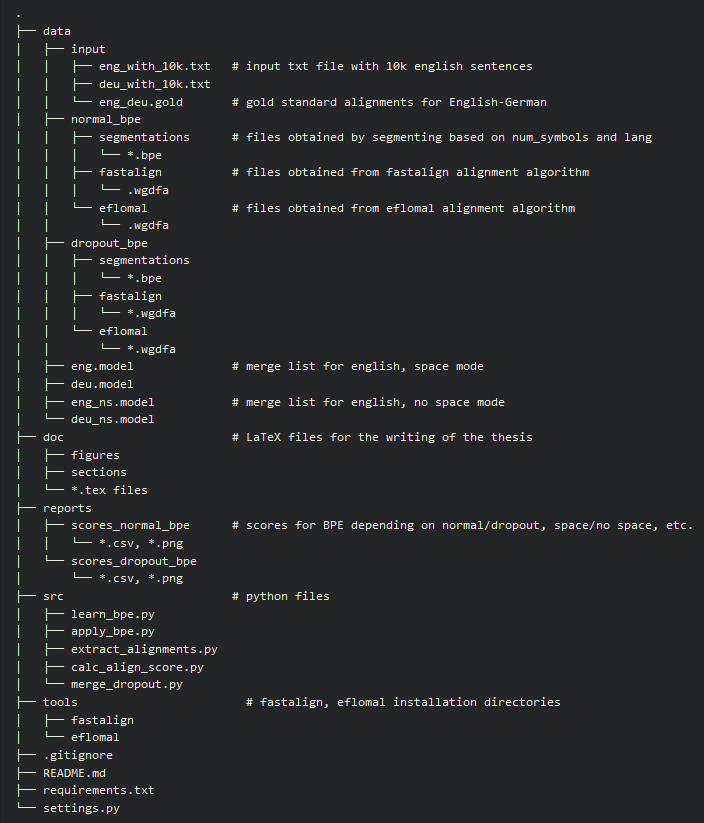
\includegraphics[width=14cm]{figures/dir.png}
    \caption{Project directories in tree mode}
\end{figure}

\clearpage
\section{Replication of BPE results}

The first programming task in this thesis has been to replicate the BPE results from Sennrich et al.~\cite{sennrich2015neural}. In order to modularize the code in clear units, these have been the steps:

\begin{enumerate}
    \item Write the learn BPE from corpus algorithm
    \item Write the apply BPE to corpus algorithm
    \item Write extract alignments script
    \item Write calculate alignment scores script
\end{enumerate}

In the following sections, each step will be explained in detail, with comments and examples for each function.

\subsection{Learn BPE algorithm}\label{subsec:learnbpe}

In learning BPE units, the first step is to read the corpus into an appropriate format. All the libraries and global variables imported are also added here for simplicity.

\begin{python}
# learn_bpe.py
import os
import re
import sys
import codecs
from os.path import join
from collections import defaultdict, Counter
# import global variables from settings.py
sys.path.insert(1, os.path.join(sys.path[0], '..'))
from settings import *

def read_corpus(corpus: list) -> list:
  '''
  Read corpus, strip index and new line characters.
  A word_sep symbol is added at the beginning of each word.
  example:
  tokens = [
      '\_w e \_d o \_n o t \_b e l i e v e 
      \_t h a t \_w e \_s h o u l d 
      \_c h e r r y - p i c k \_.',
      ...
  ]
  '''
  tokens = []
  for line in corpus:
    line = line.split('\t')[1].strip('\r\n ')
    line = line.split()
    line[0] = str.lower(line[0])

    # add word_sep to each beginning of word and join by space
    tokens.append(' '.join([word_sep + ' '.join(word) for word in line]))
  return tokens
\end{python}

Once the corpus is parsed, all pairs and their frequencies are computed and saved in a suitable data structure.

\begin{python}
# learn_bpe.py
def get_stats(tokens: list) -> Counter:
  '''
  Count frequency of all bigrams and the frequency per index.
  pairs = {
    ('s', 'h'): 5,
    ('h', 'e'): 6
  }
  The last token '.' or word_sep. is not merged with anything.
  '''
  pairs = Counter()
  for i, sent in enumerate(tokens):
    # get stats for each word independently, 
    # no bigrams between different words
    for word in sent[1:].split(' '+word_sep):
      symbols = symbols.split()
      for j in range(len(symbols) - 1):
        pairs[symbols[j], symbols[j + 1]] += 1
  return pairs
\end{python}

Following the algorithm explained in the previous chapter,~\ref{met:learnbpe}, the big/outer loop iterates between extraction of highest frequency pairs and merging of corpus until the maximum number of merges is reached.

\begin{python}
# learn_bpe.py
def merge_token(corpus: list, most_frequent: tuple) -> list:
  str_corpus = '\n'.join(corpus)
  str_corpus = str_corpus.replace(' '.join(most_frequent), ''.join(most_frequent))
  return str_corpus.split('\n')

def learn_bpe(argsinput: str) -> list:
  '''
  Learn BPE operations from vocabulary. Steps:
  1. split corpus into characters, count frequency
  2. count bigrams in corpus
  3. merge most frequent symbols
  4. Update bigrams in corpus 
  '''
  corpus = read_corpus(argsinput)
  most_frequent_merges = []
  for i in range(learn_symbols):
    pairs = get_stats(corpus)
    try:
      most_frequent = pairs.most_common(1)[0][0]
    except:
      # pairs is empty
      break
    most_frequent_merges.append(most_frequent)
    corpus = merge_token(corpus, most_frequent)
  return most_frequent_merges
\end{python}

After the loop ends, the merge list is saved into a \emph{.bpe} file. The following code includes this function as well as the main function that calls out all functions.

\begin{python}
#learn_bpe.py
def write_bpe(lang: str, most_freq_merges: list):
  bpe_file = codecs.open(join(datadir, lang+'.model'), 'w', encoding='utf-8')
  bpe_file.write(f"{lang} {len(most_freq_merges)}\n")
  bpe_file.write('\n'.join(' '.join(item) for item in most_freq_merges))
  return

if __name__ == '__main__':
  for lang in [source, target]:
    argsinput = codecs.open(inputpath[lang], encoding='utf-8')
    most_freq_merges = learn_bpe(argsinput)
    write_bpe(lang, most_freq_merges)
\end{python}

\subsection{Apply BPE algorithm}\label{dev:applybpe}

After learning BPE units, there is already a merge list written into the project data directory, which can now be loaded into memory in order to apply these merges to the corpus. The following function returns a list of the languages present in the project, BPE models and corpora for each language.

\begin{python}
# apply_bpe.py
import os
from os.path import join
import sys
import codecs
# import global variables from settings.py
sys.path.insert(1, os.path.join(sys.path[0], '..'))
from settings import *
from learn_bpe import read_bpe_model, read_corpus

def load_data() -> (list, list, list):
  langs = [source, target]
  bpe_models = []
  corpora = []
  for lang in langs:
    argsinput = codecs.open(inputpath[lang], encoding='utf-8')
    corpora.append(read_corpus(argsinput))
    bpe_model = codecs.open(join(datadir, lang+'.model'), encoding='utf-8').readlines()
    bpe_model = [tuple(item.strip('\r\n ').split(' ')) for item in bpe_model]
    bpe_models.append(bpe_model[1:])
  return langs, bpe_models, corpora
\end{python}

Once this data is available, the merge list is applied to the corpus iteratively, for the symbols present in the global variable \emph{all\_symbols}. To avoid repetition, when aiming for 8000 merges, the loop is halted at 100, 500 merges respectively, in order to save the state of the corpus into the \emph{.bpe} file. After writing the file in the system, the loop resumes again. A less efficient approach would be making the loop run until 100 merges, then start from scratch and run until 500, and so on. This method is equally effective but not nearly as efficient.

\begin{python}
# apply_bpe.py
def write_bpe(lang: str, num_symbols: int, merged_corpus: str):
  outputpath = join(bpedir, 'segmentations', f"{lang}_{num_symbols}.bpe")
  argsoutput = codecs.open(outputpath, 'w', encoding='utf-8')
  argsoutput.write(merged_corpus)
  return

def apply_bpe(langs: list, bpe_models: list, corpora: list):
  for lang, bpe_model, corpus in zip(langs, bpe_models, corpora):
    bpe_model = bpe_model[:max(all_symbols)]
    k = 0
    str_corpus = '\n'.join(corpus)
    for j, bigram in enumerate(bpe_model):
      str_corpus = str_corpus.replace(' '.join(bigram), ''.join(bigram))
      if j + 1 == all_symbols[k]:
        write_bpe(lang, all_symbols[k], str_corpus)
        k += 1
  return

if __name__ == "__main__":
  os.makedirs(join(bpedir, 'segmentations'), exist_ok=True)
  langs, bpe_models, corpora = load_data()
  apply_bpe(langs, bpe_models, corpora)
\end{python}

After this step, in the directory \emph{../data/normal\_bpe/segmentations/} various files exist with the following format:

\begin{itemize}
  \item deu\_100.bpe
  \item eng\_100.bpe
  \item deu\_200.bpe
  \item eng\_200.bpe
  \item ...
\end{itemize}

\emph{deu} or \emph{eng} refers to the language, and the numbers are the amount of merges that have been applied into this file. For examples, see~\ref{met:applybpe}.

\subsection{Extract alignments}\label{dev:extractalign}

This step requires some prior installation of the alignment software. The thesis has been conducted in a Linux environment, so the installation guide is adapted to this case. The installation of the software in any other OS is however possible, as long as the user adapts the commands to their OS. Initially, if not present in the system, it is mandatory to \href{https://cmake.org/install/}{install Cmake}. The installation steps for \emph{Fastalign} are as follows, in bash. The path \emph{path/to/project} should be the path to where the README, data folders and so on are present. Here, a new folder named \emph{tools} is created to save the alignment algorithms.

\clearpage
\begin{quote}
  sudo apt-get install libgoogle-perftools-dev libsparsehash-dev\\
  cd /path/to/project\\
  mkdir tools\\
  cd tools\\
  git clone https://github.com/clab/fast\_align.git\\
  cd fast\_align\\
  mkdir build\\
  cd build\\
  cmake ..\\
  make
\end{quote}

And for \emph{Eflomal}:

\begin{quote}
  cd /path/to/project/tools\\
  git clone https://github.com/robertostling/eflomal.git\\
  cd eflomal\\
  make\\
  sudo make install\\
  python3 setup.py install
\end{quote}

The paths for the installation are then saved in the global variable file, as well as the \emph{mode} to make the alignments, either of the two algorithms.

\begin{python}
# settings.py
mode = "fastalign" #fastalign, eflomal
fastalign_path = join(rootdir, "tools/fast_align/build/fast_align")
atools_path = join(rootdir, "tools/fast_align/build/atools")
eflomal_path = join(rootdir, "tools/eflomal")
\end{python}

In this step, as a general notion, the extract alignments script takes two files as input: English BPE file, German BPE file, and outputs an alignment file, with the extension .wgdfa. First of all, it is necessary to iterate through the different merge types that have been done before. There are BPE files with 100 merges, 200, 500, etc for both languages. At each iteration, a different alignment file is created. Regarding alignment algorithms, they work on parallel data, that is, they expect text in the following format:

\begin{quote}
  Hello from England ||| Hallo aus Deutschland
\end{quote}

Since the BPE files do not have this format, they are actually separated into two files, namely \emph{deu} and \emph{eng} files, first of all the function \emph{create\_parallel\_text} creates a \emph{.txt} file in the appropriate parallel format.

\begin{python}
# extract_alignments.py
from os.path import join
import os
import sys
import codecs
# import global variables from settings.py
sys.path.insert(1, os.path.join(sys.path[0], '..'))
from settings import *
from subword_word import *

def create_parallel_text(sourcepath: str, targetpath: str, outpath: str):
  fa_file = codecs.open(outpath + '.txt', "w", "utf-8")
  fsrc = codecs.open(sourcepath, "r", "utf-8")
  ftrg = codecs.open(targetpath, "r", "utf-8")
  for sl, tl in zip(fsrc, ftrg):
    sl = sl.strip().split("\t")[-1]
    tl = tl.strip().split("\t")[-1]
    fa_file.write(f"{sl} ||| {tl}\n")
  fa_file.close()
  return
\end{python}

\emph{Fastalign} and \emph{eflomal} work by issuing a command on the OS terminal, and they generate forward and reverse alignments. This is handled by the \emph{create\_fwd\_rev\_files} function, which creates \emph{.fwd} and \emph{.rev} files with the corresponding file name.

\begin{python}
# extract_alignments.py
def create_fwd_rev_files(outpath: str):
  if mode == "fastalign":
    os.system(f"{fastalign_path} -i {outpath}.txt -v -d -o > {outpath}.fwd")
    os.system(f"{fastalign_path} -i {outpath}.txt -v -d -o -r > {outpath}.rev")
  elif mode == "eflomal":
    os.system(f"cd {eflomal_path}; python align.py -i {outpath}.txt --model 3 -f {outpath}.fwd -r {outpath}.rev")
  return
\end{python}

Given these \emph{.fwd} and \emph{.rev} files, the alignment algorithm creates a type of union between these two, called \emph{grow-diag-final-and}, handled by the \emph{create\_gdfa\_file} function, creating files with the extension \emph{.gdfa}. The previously generated files, \emph{.fwd}, \emph{.rec}, \emph{.txt} and the intermediate file \emph{\_unnum.gdfa} are deleted from the system.

\begin{python}
# extract_alignments.py
def create_gdfa_file(outpath: str):
  # create gdfa file from .fwd and .rev
  os.system(f"{atools_path} -i {outpath}.fwd -j {outpath}.rev -c grow-diag-final-and > {outpath}_unnum.gdfa")

  # parse _unnum.gdfa to .gdfa with "\t" separator
  with codecs.open(f"{outpath}_unnum.gdfa", "r", "utf-8") as fi, codecs.open(f"{outpath}.gdfa", "w", "utf-8") as fo:
    for i, line in enumerate(fi):
      fo.write(f"{i}\t{line.strip()}\n")

  # delete unnecessary files
  os.system(f"rm {outpath}_unnum.gdfa; rm {outpath}.fwd; rm {outpath}.rev; rm {outpath}.txt")
  return
\end{python}

As explained in the \textit{Extract alignment} subsection in the Methodology chapter~\ref{subsec:extractalign}, the alignment aligns whitespace-separated units, which are generally words but in this case are subword, or BPE units. In order to actually make alignments between words, the subword alignments need to be transformed into word alignments. The function \emph{load\_and\_map\_segmentations} loads the BPE files and maps each BPE unit to its corresponding word. The comments on the function display a simple example to illustrate this concept. This is an auxiliary function in order to map the alignments later. Afterwards, by calling \emph{bpe\_word\_align}, the mapping from subword alignments to word alignments is made. Lastly, the new alignments are saved in a file with the extension \emph{.wgdfa}.

\begin{python}
# extract_alignments.py
def load_and_map_segmentations(num_symbols: int):
  '''
  Given a .bpe file composed of the corpus made of subword units such as
  corpus_eng = [
    '_We _do _no t _be li eve _.',
    '_Thi s _is _a _sent ence _.',
    ...
  ]
  Output: dictionary of each language and 
  a list of indexes pointing to which word each element (_do) belongs to
  bpes = {
    'eng':[
      [0, 1, 2, 2, 3, 3, 3, 4],
      [0, 0, 1, 2, 3, 4, 5],
      ...
    ],
    ...
  } 
  '''
  bpes = {}
  for lang in [source, target]:
    bpes[lang] = []
    corpus = codecs.open(lang+'_'+str(num_symbols)+'.bpe', encoding='utf-8')
    for sent in corpus:
      mapping = [0]
      i = 0
      for subw in sent.split()[1:]:
        if subw[0] == word_sep:
          i += 1
        mapping.append(i)
      bpes[lang].append(mapping)
  return bpes

def bpe_word_align(bpes: dict, bpe_aligns: list) -> str:
  '''
  Input: dictionary of bpes obtained as output of map_subword_to_word()
  Output: list of word alignments and their indexes
    "
      0   0-0 0-1 1-1 1-2 3-1 2-4 \n
      1   0-0 1-0 1-1 2-1 \n
      ...
    "
  '''
  all_word_aligns = ''
  for i, (sent1, sent2, bpe_al) in enumerate(zip(bpes[source], bpes[target], bpe_aligns)):
    word_aligns = set()
    # iterate each alignment
    for al in bpe_al.split('\t')[1].split():
      firstal, secondal = al.split('-')
      new_al = str(sent1[int(firstal)]) + '-' + str(sent2[int(secondal)])
      word_aligns.add(new_al)
    all_word_aligns += str(i) + "\t" + ' '.join(word_aligns) + "\n"
  return all_word_aligns
\end{python}

The alignment algorithm is executed for two types of files. Firstly, for the raw corpus itself, the alignment algorithm is executed to align the English raw corpus with the German raw corpus, which will serve as baseline to check how good the BPE merges are. And then, the alignment algorithm is executed for the BPE files themselves.

\begin{python}
# extract_alignments.py
def extract_alignments(input_mode=False: bool):
  for num_symbols in all_symbols:
    if input_mode:
      print("Alignments for input files")
      sourcepath = inputpath[source]
      targetpath = inputpath[target]
      outpath = join(bpedir, mode, "input")
    else:
      print(f"Alignments for {num_symbols} symbols")
      sourcepath = join(bpedir, 'segmentations', f"{source}_{num_symbols}.bpe")
      targetpath = join(bpedir, 'segmentations', f"{target}_{num_symbols}.bpe")
      outpath = join(bpedir, mode, str(num_symbols))
    create_parallel_text(sourcepath, targetpath, outpath)
    create_fwd_rev_files(outpath)
    create_gdfa_file(outpath)
    # map alignment from subword to word
    bpes = load_and_map_segmentations(num_symbols)
    argsalign = codecs.open(o+'.gdfa', encoding='utf-8')
    all_word_aligns = bpe_word_align(bpes, argsalign)
    os.system(f"rm {outpath}.gdfa")
    argsoutput = codecs.open(outpath+'.wgdfa', 'w', encoding='utf-8')
    argsoutput.write(all_word_aligns)
  return

if __name__ == "__main__":
  os.makedirs(join(bpedir, mode), exist_ok=True)
  if not os.path.isfile(join(bpedir, mode, 'input.wgdfa')):
    extract_alignments(input_mode=True)
  extract_alignments()
\end{python}

\subsection{Calculate alignment scores}

At this point in the pipeline, the alignments between subword units are obtained, mapped into word alignments, and the last step to be performed is to calculate the alignment scores. First of all, the gold alignment file is loaded and its alignments extracted.

\begin{python}
# calc_align_scores.py
import os
from os.path import join
import sys
import glob
import random
import collections
import pandas as pd
import matplotlib.pyplot as plt
import seaborn as sns
# import global variables from settings.py
sys.path.insert(1, os.path.join(sys.path[0], '..'))
from settings import *

def load_gold(g_path: str) -> (dict, dict, float):
  gold_f = open(g_path, "r")
  pros = {}
  surs = {}
  all_count = 0.
  surs_count = 0.
  for line in gold_f:
    line = line.strip().split("\t")
    line[1] = line[1].split()
    pros[line[0]] = set()
    surs[line[0]] = set()
    for al in line[1]:
      pros[line[0]].add(al.replace('p', '-'))
      if 'p' not in al:
        surs[line[0]].add(al)
    all_count += len(pros[line[0]])
    surs_count += len(surs[line[0]])
  return pros, surs, surs_count
\end{python}

The next function, given an input path, calculates the precision, recall, F1 and AER score based on the gold standard.

\begin{python}
# calc_align_scores.py
def calc_score(input_path: str, probs: dict, surs: dict, surs_count: float) -> (float, float, floatl float):
  total_hit, p_hit, s_hit = 0., 0., 0.
  target_f = open(input_path, "r")
  for line in target_f:
    line = line.strip().split("\t")
    if line[0] not in probs: continue
    if len(line) < 2: continue
    line[1] = line[1].split()
    for pair in line[1]:
      if pair in probs[line[0]]:
        p_hit += 1
      if pair in surs[line[0]]:
        s_hit += 1
      total_hit += 1
  target_f.close()
  y_prec = round(p_hit / max(total_hit, 1.), 3)
  y_rec = round(s_hit / max(surs_count, 1.), 3)
  y_f1 = round(2. * y_prec * y_rec / max((y_prec + y_rec), 0.01), 3)
  aer = round(1 - (s_hit + p_hit) / (total_hit + surs_count), 3)
  return y_prec, y_rec, y_f1, aer
\end{python}

This step is done for the baseline, to obtain a measure of the standard version of the system, that is, the raw English and German corpora, and then for the BPE files itself.

\begin{python}
# calc_align_scores.py
def get_baseline_score(probs: dict, surs: dict, surs_count: int) -> pd.DataFrame:
  alfile = join(bpedir, mode, 'input.wgdfa')
  score = [0]
  score.extend(list(calc_score(alfile, probs, surs, surs_count)))
  baseline_df = pd.DataFrame([score], columns=['num_symbols', 'prec', 'rec', 'f1', 'AER']).round(decimals=3)
  return baseline_df

def calc_align_scores(probs: dict, surs: dict, surs_count: int):
  scores = []
  for num_symbols in all_symbols:
    alfile = join(bpedir, mode, f"{num_symbols}.wgdfa")
    score = [int(num_symbols)]
    score.extend(list(calc_score(alfile, probs, surs, surs_count)))
    scores.append(score)
  df = pd.DataFrame(scores, columns=['num_symbols', 'prec', 'rec', 'f1', 'AER']).round(decimals=3)
  return df
\end{python}

The scores for the baseline and the corresponding BPE files are obtained and stored in a DataFrame data structure. Next, this data is plotted and saved into \emph{.png} and \emph{.csv} files.

\begin{python}
# calc_align_scores.py
def plot_scores(df: pd.DataFrame, baseline_df: pd.DataFrame, scoredir: str):
  # Use plot styling from seaborn.
  sns.set(style='darkgrid')
  # Increase the plot size and font size.
  sns.set(font_scale=1.5)
  plt.rcParams["figure.figsize"] = (12, 6)
  plt.clf()
  ax = plt.gca() # gca stands for 'get current axis'
  colors = ['magenta', 'tab:blue', 'tab:green', 'tab:red']
  df = df.sort_values('num_symbols')
  columns = list(df)
  for column, color in zip(columns[1:], colors):
    df.plot(kind='line', x=columns[0], y=column, color=color, ax=ax)
  for baseline_results, color in zip(list(baseline_df.iloc[0][1:]), colors):
    plt.axhline(y=baseline_results, color=color, linestyle='dashed')
  plt.savefig(join(scoredir+'.png'))
  return

if __name__ == "__main__":
  # Calculate alignment quality scores based on the gold standard.
  # The output contains Precision, Recall, F1, and AER.
  probs, surs, surs_count = load_gold(goldpath)
  baseline_df = get_baseline_score(probs, surs, surs_count)
  df = calc_align_scores(probs, surs, surs_count, baseline_df)
  scorename = join(scoredir, 'scores')
  print(f"Scores saved into {scorename}")
  df.to_csv(scorename+'.csv', index=False)
  plot_scores(df, baseline_df, scorename)
\end{python}

\section{Replication of BPE dropout}

The previous section has laid the backbone of the algorithms, the various files and functions. In this and the following sections, some modifications and improvements are introduced to the already existing Python scripts. For the sake of simplicity, the code snippets that follow only include the new changes, or the functions from the last section with new modifications, and the modifications are introduced by signalling the line numbers from previous scripts in which changes are introduced. For example, it might be mentioned that a certain line is added to line 21 of a certain function in a specific script. This refers to the function introduced in the previous section, and it will be referred as such. In the case that a function is altered in a significant way, the new version of the function will be shown, which overrules the previous version. The functions that remain unaltered are not shown.

When adding dropout to BPE, three new parameters come into play in the project, namely \textbf{dropout} rate, \textbf{dropout\_samples}, that is, how many samples of the dropout system are considered, and \textbf{merge\_threshold}, which serves its function with alignments later on. These values are saved into \emph{settings.py}, as well as new data directories to store files resulting from BPE dropout.

\begin{python}
# settings.py

dropout = 0.1
dropout_samples = 10
merge_threshold = [0.3, 0.5, 0.7, 0.9]

bpedir = join(datadir, 'dropout_bpe' if dropout > 0 else 'normal_bpe')
scoredir = join(rootdir, 'reports', 'scores_' + ('dropout_bpe' if dropout > 0 else 'normal_bpe'))
\end{python}

\subsection{Apply BPE to corpus with dropout}

The first modifications in the project occur in \emph{apply\_bpe.py}, where some merges are skipped, and the process is repeated 10 times. More theoretical insights regarding this approach can be found in the Methodology section~\ref{met:replbpedrop}. The function \emph{apply\_bpe} includes two new lines where a random number between 0 and 1 is generated. If this number is smaller than the \emph{dropout} rate saved in \emph{settings.py}, then that merge is not considered and the loop skips it. This means that if the \emph{dropout} variable has the value of 0.1, 10\% of merges are skipped.

Additionally, in the main function, the function \emph{apply\_bpe} is called \emph{dropout\_samples} times. To save the files accordingly, a new variable is introduced, namely \emph{i}, that does nothing in the case where dropout=0, but when repeating the process, for instance if lang=eng, num\_symbols=2000, and first iteration of dropout, that is, i=0, the files are saved as \emph{eng\_2000\_0.bpe} instead, and so on for further iterations. This is effectively achieved by changing the variable \emph{outputpath}.

In the function \emph{write\_bpe} in the general pipeline~\ref{dev:applybpe}, the following modifications are made:

\begin{python}
# apply_bpe.py
import random

def write_bpe(lang: str, num_symbols: int, merged_corpus: str, i: int =-1):
  outputpath = join(bpedir, 'segmentations', f"{lang}_{num_symbols}{f'_{i}' if i != -1 else ''}.bpe")
  argsoutput = codecs.open(outputpath, 'w', encoding='utf-8')
  argsoutput.write(merged_corpus)
  return

def apply_bpe(langs: list, bpe_models: list, corpora: list, i: int =-1):
  for lang, bpe_model, corpus in zip(langs, bpe_models, corpora):
    bpe_model = bpe_model[:max(all_symbols)]
    all_symbols_copy = all_symbols.copy()
    str_corpus = '\n'.join(corpus)
    for j, bigram in enumerate(bpe_model):
      if random.uniform(0, 1) < dropout:
        continue
      str_corpus = str_corpus.replace(' '.join(bigram), ''.join(bigram))
      if j + 1 == all_symbols_copy[0]:
        write_bpe(lang, all_symbols_copy.pop(0), str_corpus, i)
  return

if __name__ == "__main__":
  langs, bpe_models, corpora = load_data()
  if dropout > 0:
    for i in range(dropout_samples):
      apply_bpe(i)
  else:
      apply_bpe()
\end{python}

\subsection{Extract alignments with dropout}

The only change in this step is that the \emph{extract\_alignment}~\ref{dev:extractalign} function is called \emph{dropout\_samples} times, which changes the function to write the alignments in the new format, namely, changing the variables \emph{sourcepath} and \emph{targetpath}. Additionally, the gold standard's alignments do not need to be calculated since the baseline are the BPE scores rather than the gold standard scores. The rest of the alignment algorithm remains unchanged.

\begin{python}
# extract_alignments.py
# change line 2
def extract_alignments(i: int =-1, input_mode: bool =False):

# change lines 11 and 12
sourcepath = join(bpedir, 'segmentations', f"{source}_{num_symbols}_{'_'+str(i) if dropout else ''}.bpe")
targetpath = join(bpedir, 'segmentations', f"{target}_{num_symbols}_{'_'+str(i) if dropout else ''}.bpe")

# change line 30
if dropout > 0:
  for i in range(dropout_samples):
    extract_alignments(i)
else:
  extract_alignments()
\end{python}

\subsection{Calculate alignment scores with dropout}

As explained in the Methodology section~\ref{met:replbpedrop}, variants of union, intersection and threshold are created. This is introduced with a new script, namely \emph{merge\_dropout.py}. First of all, the function \emph{merge\_dropout\_alignments} opens all alignment files and creates a dictionary data structure with the union, intersection and threshold alignment files and saves them into \emph{X\_union.wgdfa}, \emph{X\_inter.wgdfa}, \emph{X\_thres.wgdfa} respectively.

\begin{python}
# merge_dropout.py
import os
from os.path import join
import sys
import codecs
import pandas as pd
from tqdm import tqdm
from collections import Counter
# import global variables from settings.py
sys.path.insert(1, os.path.join(sys.path[0], '..'))
from settings import *
from calc_align_score import *

def merge_dropout_alignments():
  union_merge, inter_merge, thres_merge = {}, {}, {}
  for num_symbols in tqdm(all_symbols, desc=f"merge_dropout: dropout={dropout}, union, inter, thres"):
    union_merge[num_symbols], inter_merge[num_symbols], thres_merge[num_symbols] = [], [], []
    for i in range(dropout_sampless):
      for j, line in enumerate(open(f'{num_symbols}_{i}.wgdfa', 'r').readlines()):
        al = frozenset(line.strip().split("\t")[1].split())

        # at the first iteration, just append the alignment
        if i == 0:
          union_merge[num_symbols].append(al)
          inter_merge[num_symbols].append(al)
          thres_merge[num_symbols].append(Counter(al))
          continue
        
        # do union, intersection or frequency addition
        union_merge[num_symbols][j] |= al
        inter_merge[num_symbols][j] &= al
        thres_merge[num_symbols][j] += Counter(al)

    # write to output
    unionfile = codecs.open(f'{num_symbols}_union.wgdfa', 'w')
    interfile = codecs.open(f'{num_symbols}_inter.wgdfa', 'w')
    thresfiles = {merge_t: codecs.open(f'{num_symbols}_thres_{merge_t}.wgdfa', 'w') for merge_t in merge_threshold}
    for i in range(len(union_merge[num_symbols])):
      unionfile.write(f"{i}\t{' '.join(union_merge[num_symbols][i])}\n")
      interfile.write(f"{i}\t{' '.join(inter_merge[num_symbols][i])}\n")
      # get alignments more common than the merge_threshold %
      for merge_t in merge_threshold:
        common_aligns = [k for k in thres_merge[num_symbols][i] 
                        if thres_merge[num_symbols][i][k] > merge_t * dropout_samples]
        thresfiles[merge_t].write(f"{i}\t{' '.join(common_aligns)}\n")
  return
\end{python}

Afterwards, the function \emph{calc\_score\_merges} opens these files and calculates the score, much in the way as the \emph{calc\_align\_score} algorithm from the previous section.

\begin{python}
def calc_score_merges():
  probs, surs, surs_count = load_gold(goldpath)
  baseline_df = pd.read_csv(join(baselinedir, f'scores_{source}_{target}.csv'))
  scorespath = join(scoredir, str(dropout))
  if not os.path.isdir(scorespath):
    os.mkdir(scorespath)

  for merge_type in ['union', 'inter']:
    scores = []
    for num_symbols in all_symbols:
      mergefilepath = join(bpedir, mode, f'{num_symbols}_{merge_type}.wgdfa')
      score = [int(num_symbols)]
      score.extend(list(calc_score(mergefilepath, probs, surs, surs_count)))
      scores.append(score)

    df = pd.DataFrame(scores, columns=['num_symbols', 'prec', 'rec', 'f1', 'AER']).round(decimals=3)
    scorename = join(scorespath, 'scores', merge_type)

    print(f"Scores saved into {scorename}")
    df.to_csv(scorename+'.csv', index=False)
    plot_scores(df, baseline_df, scorename)

  # threshold case, iterate all merge_thresholds saved
  for merge_t in merge_threshold:
    scores = []
    for num_symbols in all_symbols:
      mergefilepath = join(bpedir, mode, f'{num_symbols}_thres_{merge_t}.wgdfa')
      score = [int(num_symbols)]
      score.extend(list(calc_score(mergefilepath, probs, surs, surs_count)))
      scores.append(score)

    df = pd.DataFrame(scores, columns=['num_symbols', 'prec', 'rec', 'f1', 'AER']).round(decimals=3)
    scorename = join(scorespath, 'scores', f"{merge_t}_thres")
    
    print(f"Scores saved into {scorename}")
    df.to_csv(scorename+'.csv', index=False)
    plot_scores(df, baseline_df, scorename)
  return

if __name__ == "__main__":
    merge_dropout_alignments()
    calc_score_merges()
\end{python}

\section{Improvement of learn BPEs algorithm}\label{dev:improvbpe}

As explained in the methodology~\ref{sec:improvlearnbpe}, the main improvement in the learn-BPE algorithm is to only update previous and next tokens to the merged pair, as well as saving the indexes where each pair occurs. These improvements are built on top of the code shown in~\ref{subsec:learnbpe}. 

In the \emph{learn\_bpe} function, the new \emph{update\_tokens} returns the updated pairs and the merged tokens, all in one step. The function \emph{get\_stats}, which is the function that iterates the whole corpus, only has to be performed once. This is however a modification of the previous \emph{get\_stats} function, since it computes the indexes of the pairs as well.

\begin{python}
def learn_bpe(corpus: list, bpe_model: list): list:
  '''
  Learn BPE operations from vocabulary.
  Steps:
  1. split corpus into characters, count frequency
  2. count bigrams in corpus
  3. merge most frequent symbols
  4. Update bigrams in corpus 
  '''
  tokens = read_corpus(corpus)
  pairs, idx = get_stats(tokens)
  most_frequent_merges = []
  for i in range(learn_symbols):
    try:
      most_frequent = pairs.most_common(1)[0][0]
    except:
      # pairs is empty
      break
    most_freq_merges.append(most_frequent)
    tokens, idx, pairs = update_tokens(tokens, idx, pairs, most_frequent)
  return most_freq_merges
\end{python}

These are the modifications introduced in the \emph{get\_stats} function so that it saves the pair indexes. In the \emph{idx} data structure, not only is the index saved, but also the amount of appearances of each pair in that sentence. This is done to ensure that if the pair ('t', 'h') in index 0 now becomes ('t', 'he') because of the ('h', 'e') merge, and the frequency of ('t', 'h') is reduced by one, it might be assumed that ('t', 'h') no longer appears in that sentence. But this would be a mistake, since there might be other instances of ('t', 'h') in the sentence that are not altered by this merge. We only want to say that ('t', 'h') no longer appears in index 0 when all instances of ('t', 'h') have been merged with other sequences. This is the motivation behind storing the amount of appearances of each pair in a sentence.

\begin{python}
# learn_bpe.py
def get_stats(tokens: list) -> (Counter, dict):
  """
  Count frequency of all bigrams, the indexes where they occur and the frequency per index.
  pairs = {
      ('s', 'h'): 5,
      ('h', 'e'): 6
  }
  idx = {
      ('t', 'h'): {
          # keys are indexes in corpus, values are frequency of appearance
          0: 2,
          1: 3,
      }
  }
  """
  def get_pairs_idx(pairs, idx, symbols):
    symbols = symbols.split()
    for j in range(len(symbols) - 1):
      new_pair = symbols[j], symbols[j + 1]
      pairs[new_pair] += 1
      idx[new_pair][i] += 1
    return pairs, idx

  pairs = Counter()
  idx = defaultdict(lambda: defaultdict(int))
  for i, sent in enumerate(tokens):
    # get stats for each word independently, no bigrams between different words
    for word in sent[1:].split(' '+word_sep):
      pairs, idx = get_pairs_idx(pairs, idx, word_sep + word)
  return pairs, idx
\end{python}

The \emph{update\_tokens} function handles the situation where only the previous and after tokens are updated for each merged pair. Comments are included in the code for readability.

\begin{python}
# learn_bpe.py
def update_tokens(tokens, idx, pairs, pair):

  def update_freqs(pairs, idx, pair, new_pair=-1):
    # decrease freq from pairs
    pairs[pair] -= 1
    if pairs[pair] <= 0: del pairs[pair]
    # decrease freq from idx
    idx[pair][i] -= 1
    if idx[pair][i] <= 0: del idx[pair][i]
    if len(idx[pair]) <= 0: del idx[pair]
    if new_pair != -1:
      pairs[new_pair] += 1
      idx[new_pair][i] += 1
    return pairs, idx

  merged_pair = ''.join(pair)
  p = re.compile(r'(?<!\S)' + re.escape(' '.join(pair)) + r'(?!\S)')
  # only iterate the corpus indexes where the pair to be merged is present
  for i in list(idx[pair]).copy():

    # merge pair in the sentence
    sent = p.sub(merged_pair, tokens[i])
    # sentence remains unchanged. Delete pair from pairs and idx and continue
    if sent == tokens[i]:
      del pairs[pair]
      del idx[pair][i]
      if len(idx[pair]) <= 0:
        del idx[pair]
      continue
    tokens[i] = sent
    '''
    iterate sent by the position the merged_pair occurs. 
    in each position, we need to reduce freq of previous and after tokens
    sentence before merge: 'h e l l o', pair: ('e', 'l')
    merged sent = 'h el l o'
    sent.split(merged_pair) -> ['h ', ' l o']
    we iterate the splitted sentence and in each occasion
    * decrease freq of previous token ('h', 'e')
        * create new token ('h', 'el')
    * decrease freq of after token ('l', 'l')
        * create new token ('el', 'l')
    * decrease freq of merged pair ('e', 'l')
    '''
    sent = sent.split(merged_pair)
    for k in range(len(sent[:-1])):
      if sent[k].split() and sent[k][-1] == ' ' and word_sep not in pair[0][0]:
        '''
        conditions to update the **previous** token:
        * if sent[k] is not empty. if it is, there's no previous token to update.
        * if the merged_pair is not the beginning of the word.
          * in this case, we do not want the last letter from the prev word to be merged with
          * our current pair. ... e _t h ... we do not want to consider ('e', '_t')
        '''
        prev = (sent[k].split()[-1], pair[0])
        new_pair = (prev[0], merged_pair)
        pairs, idx = update_freqs(pairs, idx, prev, new_pair)

      if not sent[k+1].split() and word_sep not in pair[0][0]:
        '''
        conditions to update the **after** token when merged bigrams are consecutive:
        * when the pair's first character is not the beginning of the word
        * and when the next token is empty
        * we're dealing with consecutive merged pairs, merged_pair = ('ssi'), sent= 'm i ssi ssi p p i'
            * in this case, we delete the token between the merged_pair: ('i', 's')
            * and create a new pair ('ssi', 'ssi')
        '''
        if sent[k] and sent[k][-1] == word_sep:
          after = (word_sep+merged_pair, pair[0])
          new_pair = -1
        else:
          after = (pair[1], pair[0])
          new_pair = (merged_pair, merged_pair)
          pairs, idx = update_freqs(pairs, idx, after, new_pair)
      elif sent[k+1].split() and word_sep not in sent[k+1].split()[0]:
        '''
        conditions to update the **after** token in a more general case:
        * if sent[k] is not empty. if it is, there's no after token to update.
        * if the after token is a new word, we do not want to consider it.
        '''
        after = (pair[1], sent[k+1].split()[0])
        new_pair = (merged_pair, after[1])
        pairs, idx = update_freqs(pairs, idx, after, new_pair)
      # decrease freq of merged bigram
      pairs, idx = update_freqs(pairs, idx, pair)
  return tokens, idx, pairs
\end{python}

The performance improvements of this approach can be seen in the Results section.

\section{BPE without word boundaries}

As explained in the Methodology chapter, this addition considers BPE units between different words. The only change occurs when learning these BPE units and mapping multiple-word-units to multiple-word-units, the rest of the pipeline remains as is, other than changing the filenames and paths of the alignments and scores. A new Boolean variable is introduced in \emph{settings.py}, so that by changing it to a positive value will make the whole pipeline act in space mode, that is, setting the space boundary and only allowing merges between words. On the contrary, no space mode allows merges between different words.

\begin{python}
# settings.py
space = False
\end{python}

The following scripts for learning BPEs and extracting and mapping alignments are generalized in the sense that just by changing the Boolean variable in the settings file, the pipeline runs automatically and no further changes need to be done. The code snippets below display these functionality, accepting both modes.

In \emph{learn\_bpe.py}, the way to parse and tokenize the corpus is slightly different, now instead of having a special token to denote the beginning of a word, the special token denotes the whitespace.

\begin{python}
# learn_bpe.py
def read_corpus(corpus: list) -> list:
  '''
  Read corpus, strip index and new line characters.
  In space mode, each word has a word_sep symbol at the beginning to signal it is the beginning of the word.
  tokens = [
    'w e \_d o \_n o t \_b e l i e v e \_t h a t \_w e \_s h o u l d \_c h e r r y - p i c k \_.',
  ]
  In no space mode, there's no signal at the beginning of the word but word are joined by word_sep.
  tokens = [
    'w e \_ d o \_ n o t \_ b e l i e v e \_ t h a t \_ w e \_ s h o u l d \_ c h e r r y - p i c k \_ .',
  ]
  '''
  tokens = []
  for line in corpus:
    line = line.split('\t')[1].strip('\r\n ')
    line = line.split()
    line[0] = str.lower(line[0])
    if space:
      # add word_sep to each beginning of word and join by space
      tokens.append(' '.join([word_sep + ' '.join(word) for word in line]))
    else:
      # join all words by word_sep
      tokens.append(u' \u2581 '.join([' '.join(word) for word in line]))
  return tokens
\end{python}

When analysing pairs and their frequencies, each word's last character and the following whitespace has to be considered, as well as this whitespace and the following word's first character. This changes the \emph{get\_stats} function slightly.

\begin{python}
# learn_bpe.py
def get_stats(tokens: list) -> (Counter, dict):
  '''
  Count frequency of all bigrams, the indexes where they occur and the frequency per index.
  pairs = {
    ('s', 'h'): 5,
    ('h', 'e'): 6
  }
  idx = {
    ('t', 'h'): {
        # keys are indexes in corpus, values are frequency of appearance
        0: 2,
        1: 3,
    }
  }
  In space mode, the last token '.' or word_sep. is not merged with anything.
  '''
  def get_pairs_idx(pairs, idx, symbols):
    symbols = symbols.split()
    for j in range(len(symbols) - 1):
      new_pair = symbols[j], symbols[j + 1]
      pairs[new_pair] += 1
      idx[new_pair][i] += 1
    return pairs, idx

  pairs = Counter()
  idx = defaultdict(lambda: defaultdict(int))
  for i, sent in enumerate(tokens):
    if space:
      # get stats for each word independently, no bigrams between different words
      for word in sent[1:].split(u' \u2581'):
      pairs, idx = get_pairs_idx(pairs, idx, word_sep + word)
    else:
      # get bigram stats for the whole sentence
      pairs, idx = get_pairs_idx(pairs, idx, sent)
  return pairs, idx
\end{python}

And finally, after merging a pair in the corpus, when updating the tokens and the pairs, the fact that space boundaries exist or not also plays a role. Specifically, the no space mode enjoys more freedom, in the sense that no matter which pair is merged, the pair immediately before and the pair immediately after are merged, no matter what. In space mode however, this cannot be done if the previous or next pair belong to another word, which puts some restrictions. Only modified lines with respect to the code in the previous improve learn BPE algorithm~\ref{dev:improvbpe}. There are comments in the code for readability.

\begin{python}
# learn_bpe.py
def update_tokens(tokens: list, idx: dict, pairs: Counter, pair: tuple) -> (list, dict, Counter):

# change line 46
if sent[k].split() and (sent[k][-1] == ' ' and word_sep not in pair[0][0] if space else True):
  '''
  conditions to update the **previous** token:
  * in space mode, if the merged_pair is not the beginning of the word.
    * in this case, we do not want the last letter from the prev word to be merged with
    * our current pair. ... e _t h ... we do not want to consider ('e', '_t')
  '''

# change line 58
if space and not sent[k+1].split() and word_sep not in pair[0][0]:
  '''
  conditions to update the **after** token when merged bigrams are consecutive:
  * in space mode specifically, when the pair's first character is not the beginning of the word
  '''

# change line 74
elif sent[k+1].split() and (word_sep not in sent[k+1].split()[0] if space else True):
  '''
  * in space mode, if the after token is a new word, we do not want to consider it.
  '''
\end{python}

The \emph{apply\_bpe.py} remains unchanged, aligning BPE files as well with the \emph{Fastalign} or \emph{Eflomal} algorithm as well. However, since now the alignments are among many words, the mapping is different than in the space case. The mapping is divided into subword to word mapping (map\_subword\_.to\_word function) and multiword to word (map\_multiword\_to\_word).

\begin{python}
# extract_alignments.py
def map_subword_to_word(corpus, bpes, lang):
  '''
  SPACE MODE
  Input: list of sentences with subword separation
  corpus =  [
    '_We _do _no t _be li eve _.',
    '_Thi s _is _a _sent ence _.',
  ]
  Output: dictionary of each language and 
  a list of indexes pointing to which word each element (_do) belongs to
  bpe = {
    source:
    [
      [0, 1, 2, 2, 3, 3, 3, 4],
      [0, 0, 1, 2, 3, 4, 5],
    ],
  }
  '''
  bpes[lang] = []
  for sent in corpus:
    mapping = [0]
    i = 0
    for subw in sent.split()[1:]:
      if subw[0] == word_sep:
        i += 1
      mapping.append(i)
    bpes[lang].append(mapping)
  return bpes
\end{python}

And the new \emph{map\_multiword\_to\_word} function.

\begin{python}
# extract_alignments.py
def map_multiple_to_word(corpus, bpes, lang):
  '''
  NO SPACE MODE
  Input: list of sentences with subword separation
  corpus =  [
    'b u t_this_is_no t_w hat_hap pen s_.',
    'th e_ ice_cre am_.',
  ]
  Output: dictionary of each language and 
  a list of indexes pointing to which word each element (t\_w) belongs to
  bpes = {
    source:
    [
      [[0], [0], [0,1,2,3], [3,4], [4,5], [5], [5,6]],
      [[0], [0], [1,2], [2]],
    ],
  }
  '''
  bpes[lang] = []
  for sent in corpus:
    sent_bpes = []
    j = 0
    for word in sent.split():
      if word == word_sep:
        # word is simply '_', doesn't belong to anything
        j += 1
        sent_bpes.append([])
        continue
      word_count = word.count(word_sep)
      if word_count == 0:
        sent_bpes.append([j])
        continue
      # multiple words in the element: t_this_is_no -> [0,1,2,3]
      if word[0] == word_sep:
        # word starts with '_' but there are no elements of the previous word in it
        j += 1
        word_count -= 1
      if word[-1] == word_sep:
        # word ends with '_' but there are no elements of the next word in it
        sent_bpes.append(list(range(j, j + word_count)))
      else:
        sent_bpes.append(list(range(j, j + word_count + 1)))
      j += word_count
    bpes[lang].append(sent_bpes)
  return bpes
\end{python}

Consequently, the function \emph{load\_and\_map\_segmentations} is altered in the following way:

\begin{python}
# extract_alignments.py
def load_and_map_segmentations(num_symbols, i=-1):
  bpes = {}
  for lang in [source, target]:
    segmentpath = lang+'_'+str(num_symbols)+('_'+str(i) if i != -1 else '')+'.bpe'
    argsinput = codecs.open(segmentpath, encoding='utf-8')
    if space:
        bpes = map_subword_to_word(argsinput, bpes, lang)
    else:
        bpes = map_multiple_to_word(argsinput, bpes, lang)
  return bpes
\end{python}

Besides, the function \emph{bpe\_word\_align} is also altered to account for the fact that if a multiword unit such as \emph{from\_the} is aligned with \emph{aus\_dem}, each one-to-one alignment must be considered, that is, from-aus, from-dem, the-aus, and the-dem.

\begin{python}
def bpe_word_align(bpes, bpe_aligns):
  '''
  Input: dictionary of bpes obtained as output of map_subword_to_word()
  Output: list of word alignments and their indexes
    "
      0   0-0 0-1 1-1 1-2 3-1 2-4 \n
      1   0-0 1-0 1-1 2-1 \n
    "
  '''
  all_word_aligns = ''
  for i, (sent1, sent2, bpe_al) in enumerate(zip(bpes[source], bpes[target], bpe_aligns)):
    word_aligns = set()
    # iterate each alignment
    for al in bpe_al.split('\t')[1].split():
      firstal, secondal = al.split('-')
      if space:
        new_al = str(sent1[int(firstal)]) + '-' + str(sent2[int(secondal)])
        word_aligns.add(new_al)
      else:
        for el1 in sent1[int(firstal)]:
          for el2 in sent2[int(secondal)]:
            new_al = str(el1) + '-' + str(el2)
            word_aligns.add(new_al)
    all_word_aligns += str(i) + "\t" + ' '.join(word_aligns) + "\n"
  return all_word_aligns
\end{python}

The final step of calculating scores does not change.
